\chapter{Figure Supplements}
\label{supplements}
\bibliographystyle{nar}
%\section{Supplement Figures for Chapter 2}
\begin{figure}
\centering
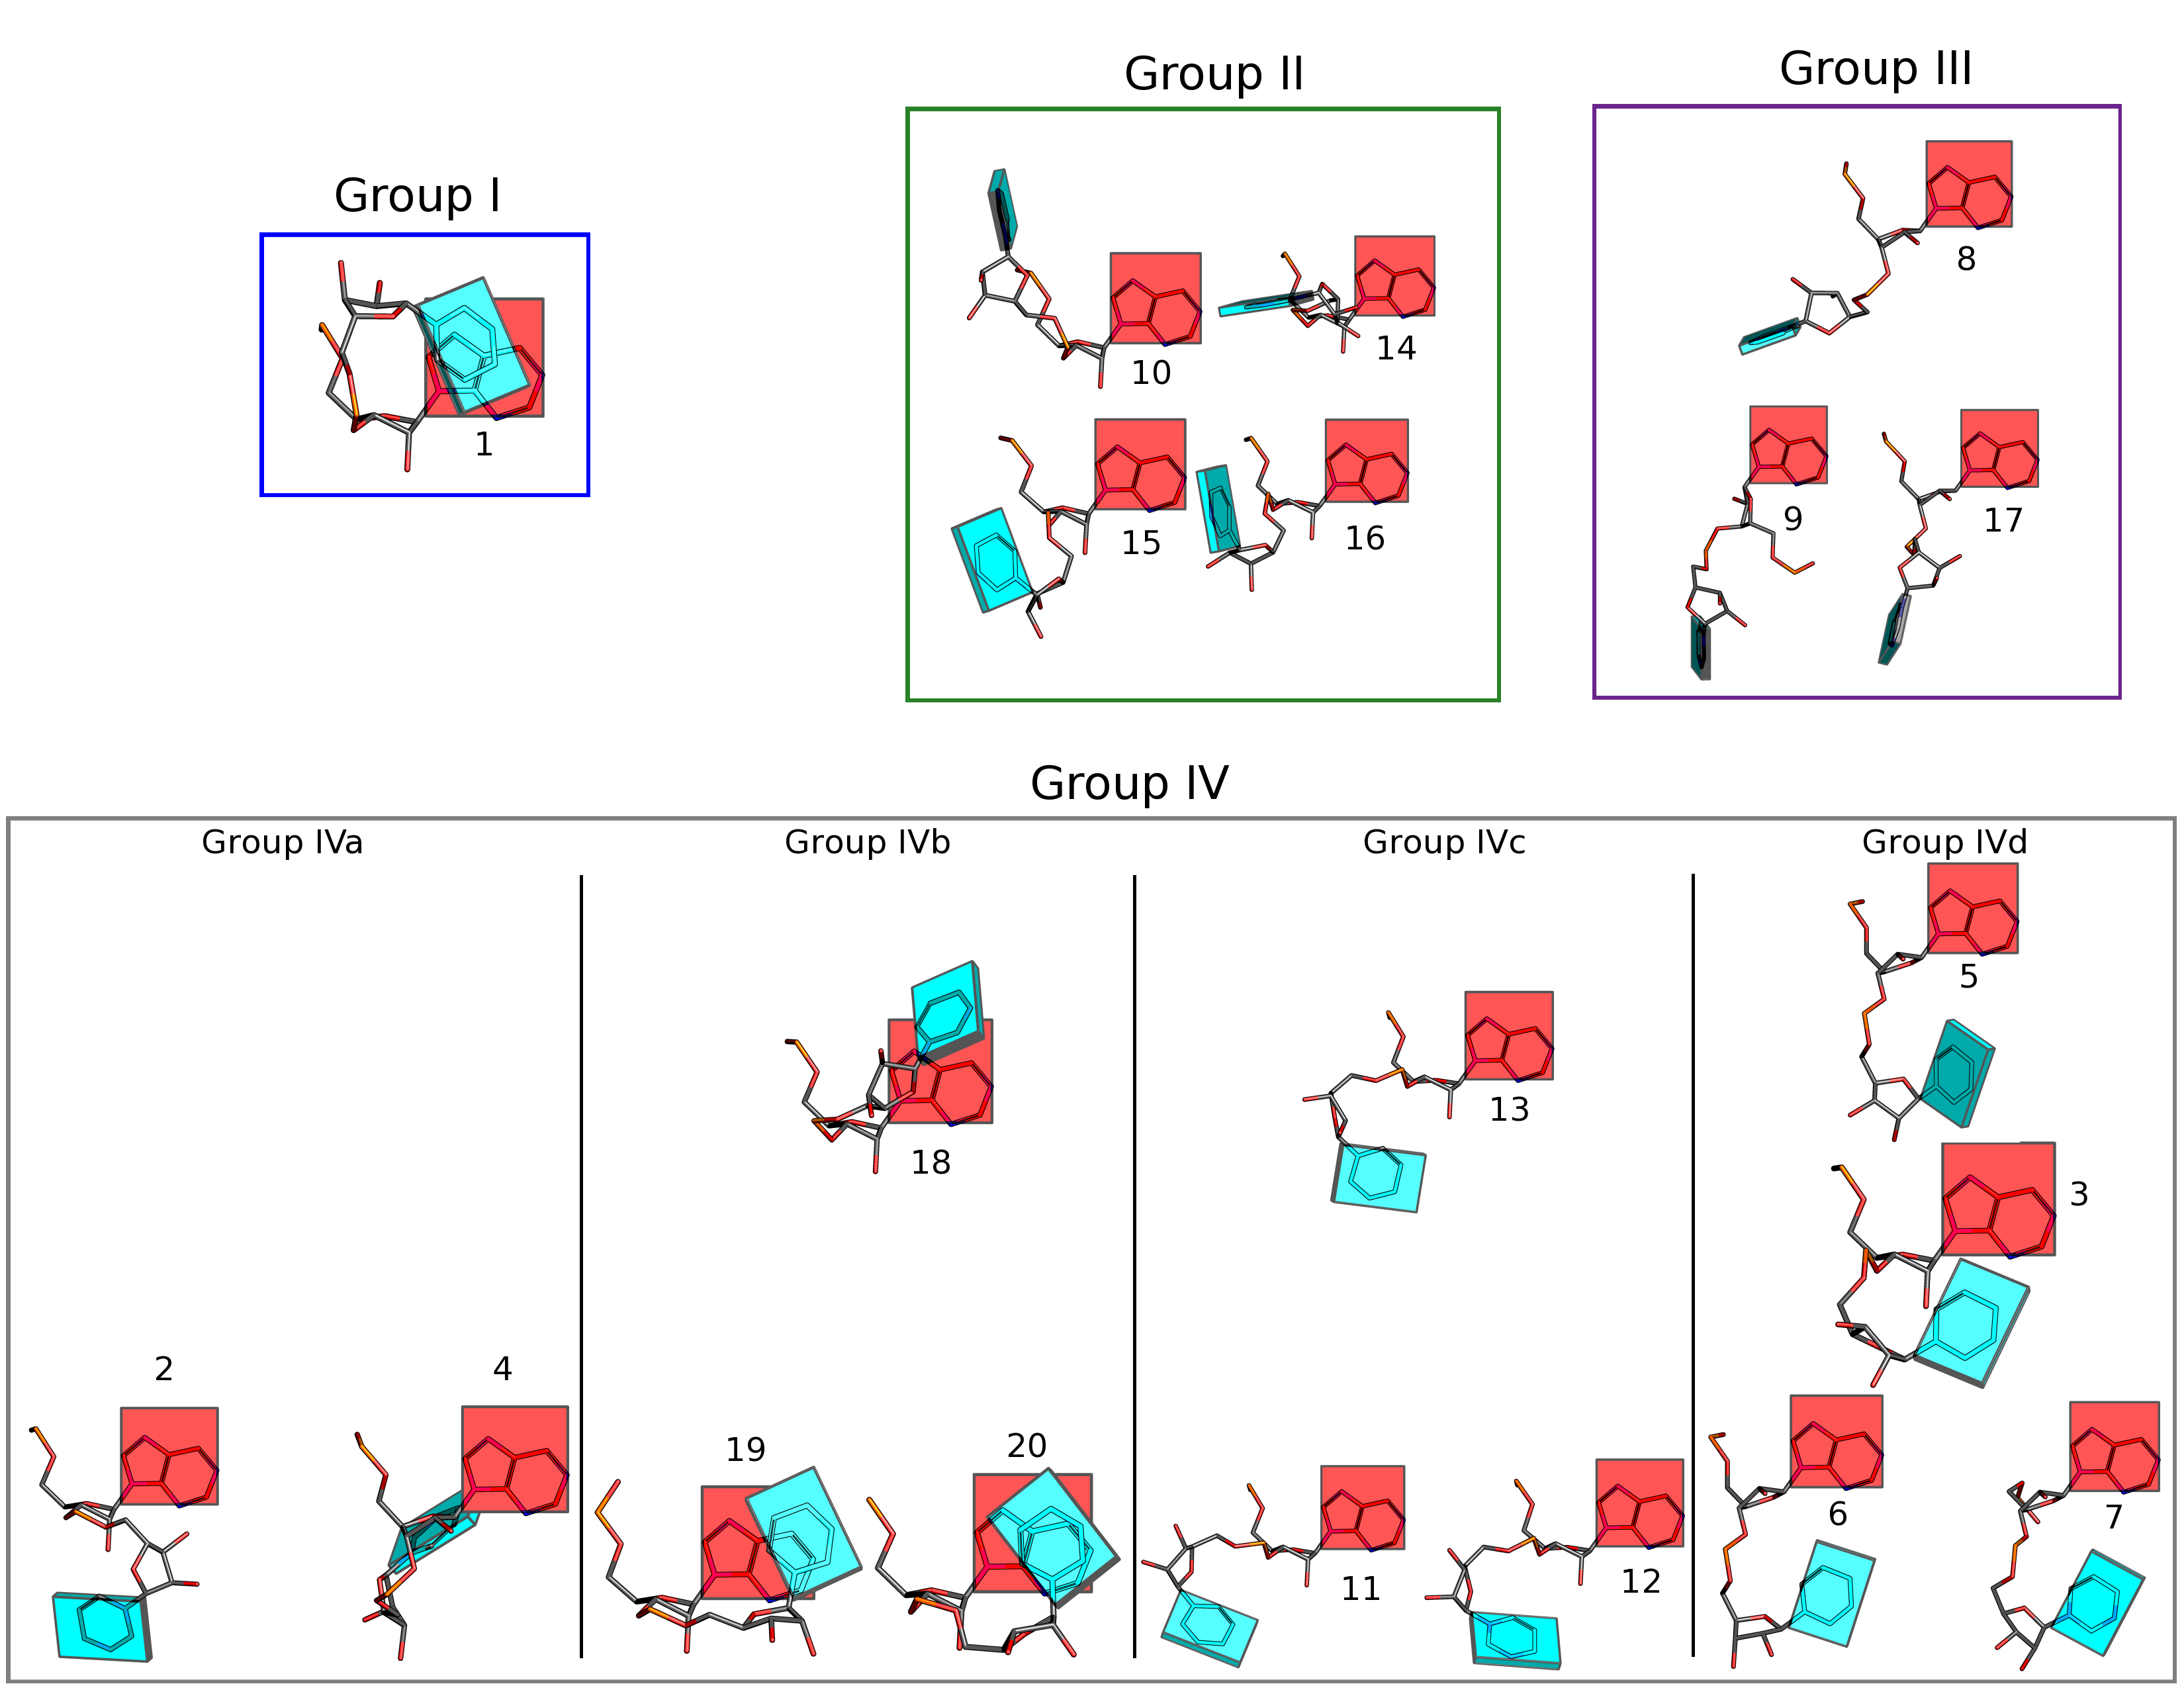
\includegraphics[angle=90, scale=0.5]{Supplement/collage2.png}
\caption{Non A-RNA Type base steps centered on the standard reference
  frame of Adenine. Top view with the Minor Groove side of Adenine
  pointing down the page and the Major Groove pointing up.}
\label{fig:steps2}
\end{figure}

\begin{figure}
\centering
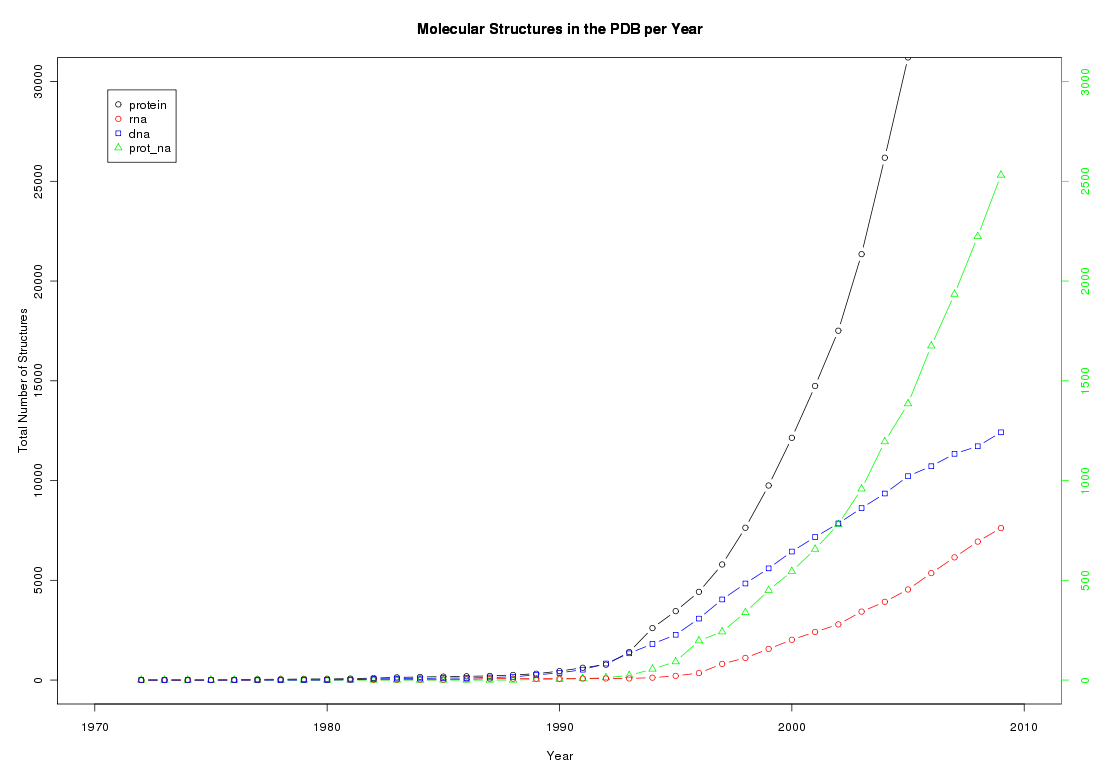
\includegraphics[angle=90, scale=0.5]{Supplement/allmolecules_per_year.png}
\caption{The total number of structures available in the pdb up to the
end of year 2009. The scale of the axis in the left (in black), is ten
times that in the right (in green). The black y-axis sets the scale
for the number of protein structures available in the PDB up to the
end of the year 2009. The green y-axis sets the scale for the number
of molecular structures containing, rna only (in red), dna only (in
blue), and protein plus nucleic acid (in green).
One can clearly see that the total number of protein, rna, and protein
plus nucleic acid structures is growing exponentially. It is also
clear that the number of DNA structures is perhaps tending toward a
constant number, that is, it might not be growing. It is also
interesting to see how the number of RNA structures really lifts off in the
middle of the nineties, whereas for DNA the growth started earlier and
is settling down.}
\label{fig:allpolypdb}
\end{figure}

\bibliography{biblio}


